% !TEX root = domain_transduction.tex
We address the problem of unsupervised transductive domain adaptation by jointly solving for the label assignment of unsupervised target domain as well as the shift between the domains. We first define our model in Section~\ref{prob:def} and explain the two sub-problems of transduction and adaptation. We further explain the details of transduction in Section~\ref{label} and the details of adaptation in Section~\ref{metric}.
%Unsupervised domain adaptation is inherently a transduction problem since the main challenge lies in labeling the unsupervised data points with the help of the supervised data; because, adaptation is done offline without computationally concerns and the accuracy is critical since the transduction error is a good proxy for generalization \cite{adapttheory}. Main complication, which makes existing transduction methods inapplicable, is the domain shift between the supervised and unsupervised data points . We explicitly model the domain shift and jointly solve for unsupervised labels as well as the domain shift in a transductive learning setup.

\subsection{Problem Definition}
\label{prob:def}
In the unsupervised domain adaptation problem, one of the domains (source) is fully supervised $\{\xsi, \ysi \}_{i \in [N^s]}$ with $N^s$ data points $\xsi$ and corresponding labels $\ysi$ from a discrete set $\ysi \in \{1,\ldots, k \}$.  The other domain (target), on the other hand is unsupervised and has $N^u$ data points $\{\xui \}_{i \in [N^u]}$. 

We further assume that both domains have different distributions $\xsi \sim p_s$ and $\xui \sim p_t$ defined on the same space as $\xsi,\xui \in \mathcal{X}$ and there exists a feature function \mbox{$\Phi:\mathcal{X}\rightarrow \mathcal{R}^d$} which is applicable to both. We further study the case where the feature function is parametric with a parameter $\mathbf{\theta}$ defined as \mbox{$\Phi_\mathbf{\theta}:\mathcal{X}\rightarrow \mathcal{R}^d$}, and we develop a method to learn the parameters.

Our model has two main components, transduction and adaptation. The transduction is the sub-problem of labelling unsupervised data points and the adaptation is solving for the domain shift. 

For adaptation, we explicitly model the domain shift in the form of an asymmetric similarity as
\begin{equation}
\sw(\xsi,\xuj) = \Phi(\xsi)^\intercal \mathbf{W} \Phi(\xuj)
\end{equation}
such that it is high if two data points, $\xsi$ from the source and $\xuj$ from the target, are from the same class.

We further model our transduction in the form of a nearest neighbor and we follow the triplet loss defined in \cite{lmnn} in order to solve adaptation by taking the nearest neighbor inference into learning. While the original triplet loss \cite{lmnn} enforces a margin $\alpha$ between the similarity of any point to its nearest neighbor from the same class and the nearest neighbor from other classes, we extend this construction to the unsupervised domain adaptation by enforcing a similar margin. For each source point, we enforce a margin between its similarity with the nearest neighbor from the target having the same label and having a different label as; $ \sw(\xsi,\mathbf{x}_{i^+}) > \sw(\xsi,\mathbf{x}_{i^-}) + \alpha$ where $\mathbf{x}_{i^+}$ is the nearest target having the same class as $\xsi$ and $\mathbf{x}_{i^-}$ is the nearest target having a different class label.

Since we model our problem as transduction, we include target labels as part of the joint learning and introduce a target label consistency term as well. We enforce that similar unsupervised data points should have the same label after the transduction by penalizing label disagreements between similar images.

Our model leads to the following optimization problem, over the target labels $\yui$ and the similarity metric $\mathbf{W}$, jointly solving transduction and adaptation. 
\begin{equation}
\begin{aligned}
\min_{\mathbf{W}, y_1, \ldots y_{N^u}} &\sum_{i \in [N^s]} &&[\sw(\xsi,\mathbf{x}_{i^-}) - \sw(\xsi,\mathbf{x}_{i^+}) + \alpha]_{+}  \\
&+\lambda &&\hspace{-3mm}\sum_{i \in N^u} \sum_{j \in \mathcal{N}(\xui)}  sim(\xui, \xuj) \mathds{1}(y_i \neq y_j)\\
% \Phi(\xui)^\intercal \Phi(\xuj) \mathds{1}(y_i \neq y_j)\\
&s.t. \quad &&i^{+} = {\arg\max}_{j | y_j = \hat{y}_i} \sw(\mathbf{\hat{x}}_i,\mathbf{x}_{j}) \\
&\quad &&i^{-} = {\arg\max}_{j | y_j \neq \hat{y}_i} \sw(\mathbf{\hat{x}}_i,\mathbf{x}_{j}) 
\end{aligned}
\label{loss}
\end{equation}
where $\mathds{1}(a)$ is an indicator function which is $1$ if $a$ is true and $0$ otherwise. $[a]_+$ is a rectifier function which is equal to $\max(0, a)$, and $sim$ is any similarity function. We use cosine similarity as $sim(\xui, \xuj)= \frac{\Phi(\xui)^\intercal \Phi(\xuj)}{|\Phi(\xui)||\Phi(\xuj)|}$. 

We solve this optimization problem via alternating minimization through iterating over solving for unsupervised labels $y_i$(transduction) and learning the similarity metric $\mathbf{W}$ (adaptation). We explain these two steps in detail in the following sections.

 
 %} $ 

%$\max_{y_1} \$
%$\min_{y_1} + 
%_4) $ assuming green is $0$, blue is $1$ and red is $2$

\subsection{Transduction: Labeling Target Domain}
\label{label}
\begin{figure}[ht]
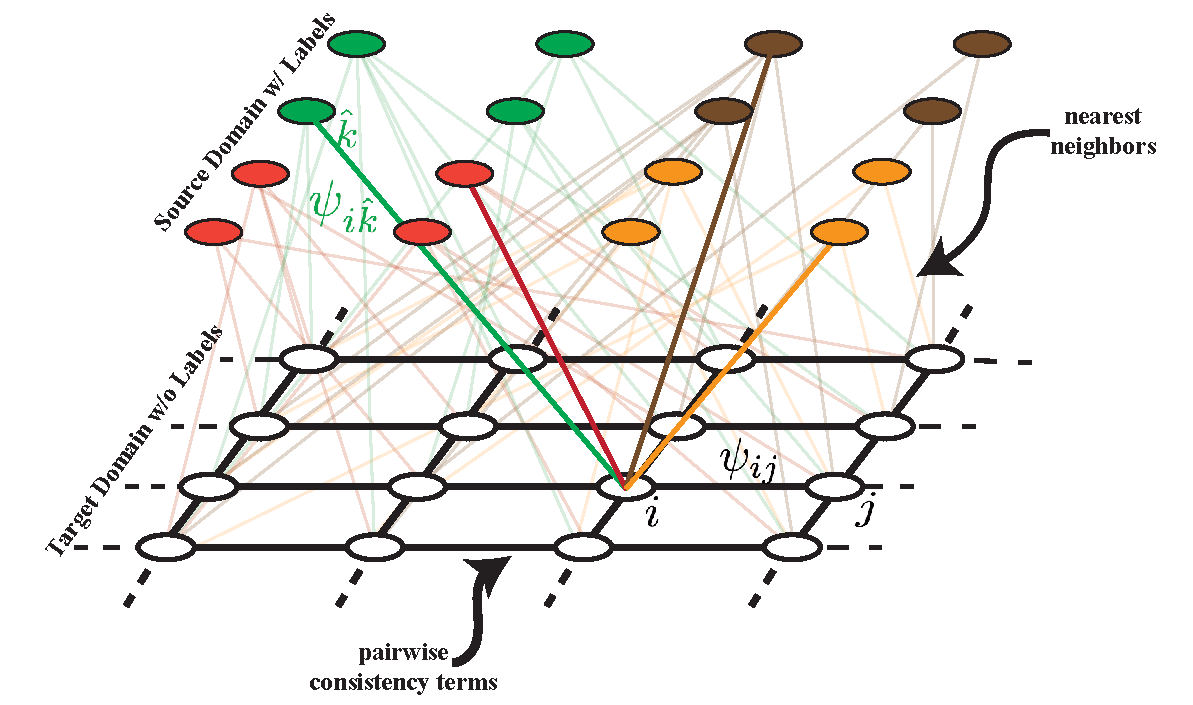
\includegraphics[width=\columnwidth]{fig11}
\vspace{-6mm}
\caption{\textbf{Visualization of the Label Propogation.} We create a k-NN graph of unsupervised target points to enforce consistency with pairwise terms 
\mbox{$\psi_{ij}=sim(\mathbf{x}_i, \mathbf{x}_j) \mathds{1}(y_i \neq y_j)$} and use closest supervised source points to each class as 
\mbox{$ \psi_{i\hat{k}} \sw(\mathbf{\hat{x}}_k,\mathbf{x}_{i})$}.} 
\label{vis_label_prop}
\end{figure}
In order to label the unsupervised points, we use the nearest-neighbor rule. We simply compute the NN supervised data point for each unsupervised data point using the learned metric $\sw(\cdot,\cdot)$ and transfer the corresponding label. In the initial stages of our optimization, our tranduction needs to be accurate even with a sub-optimal similarity metric due to the iterative fashion of our algorithm. Hence, we enforce a consistent labeling via label propagation. We first formally define the NN-rule and then introduce the label propagation.

Given a similarity metric $\sw(\cdot,\cdot)$, the NN rule is:
\begin{equation}
(y_i)^{pred} = \hat{y}_{{\arg\max}_j \sw(\mathbf{x_i}, \mathbf{\hat{x}_j})}
\end{equation}

We use label propagation to enforce consistency of the predicted labels of unsupervised data points. Our label propagation is similar to existing graph transduction algorithms \cite{label_prop1,label_prop2}. In order to enforce this consistency, we create a k-nearest neighbor (k-NN) graph over the unsupervised data points such that neighbors $\mathcal{N}(\xui)$ for $\xui$ is the k-unsupervised data point having highest similarity to $\xui$ using the cosine similarity in the feature space. After the k-NN graph is created, we solve the following optimization problem for labeling unsupervised data points with label propagation:
\begin{equation}
\begin{aligned}
\min_{y_1, \ldots y_{N^u}}  &\sum_{i \in N^u} - \max_{\hat{y}_j=y_i}  \sw(\mathbf{\hat{x}}_j,\mathbf{x}_{i}) \\
&+ \lambda
\sum_{i \in N^u} \sum_{j \in \mathcal{N}(\mathbf{x}_i)} sim(\mathbf{x}_i, \mathbf{x}_j) \mathds{1}(y_i \neq y_j)
\end{aligned}
\label{robtran}
\end{equation}
This problem can approximately be solved using many existing methods such as $\alpha$-$\beta$ swapping, quadratic pseudo-boolean optimization (QPBO) and linear programming through roof-duality. We use the $\alpha$-$\beta$ swapping algorithm from \cite{kolmogrovalphabeta} since it is experimentally shown to be efficient and accurate. In order to further explain the label propagation, we visualize an example with $k=4$ and $4$-class classification problem in Figure~\ref{vis_label_prop}. 

It is also critical that this formulation requires solving high number of nearest neighbors which is computationally challenging. However, our choice of optimization method makes this computation tractable. We use stochastic gradient descent in our adaptation stage with a carefully chosen batch size, which requires us to only solve the transduction over a batch. %Furthermore, we also efficiently implement the distance computation in the form of a few OpenBLAS calls as we further explain in detail in Section~\ref{imp_det}.

\subsection{Adaptation: Learning the Metric}
\label{metric}
Given the predicted labels $y_i$ for unsupervised data points $\xui$, we need to learn an asymmetric metric in order to minimize the loss function defined in (\ref{loss}). 

The main intuition behind our formulation is to seek a metric which can label the supervised points correctly using the unsupervised points and their predicted labels. In other words, we reverse the labeling direction. At this stage we have already predicted a label for each unsupervised point; hence, we can estimate a label for each supervised point using the predicted labels. We also have ground truth labels for the supervised points and we combine them to find an asymmetric metric. In other words, the goal of the adaptation stage is:

\vspace{-3mm}
\begin{itemize}
\item predicting $\hat{y}^{pred}_j$ using $\xui, \xsj, \yui$
\item learning $\sw(\cdot,\cdot)$ by penalizing  $(\hat{y}_j)^{pred} \neq \hat{y}_j$ 
\end{itemize}

Fortunately, this can be jointly solved by minimizing the triplet loss defined with supervised data points and their closest same class and different class neighbors among the unsupervised points. Formally, we find the closest same class and different class points as;
\begin{equation}
\begin{aligned}
&i^{+} = {\arg\max}_{j | y_j = \hat{y}_i} \sw(\xsi, \xui) \\
&i^{-} = {\arg\max}_{j | y_j \neq \hat{y}_i} \sw(\xsi,\xuj) 
\label{sup_nn}
\end{aligned}
\end{equation}

We further define the loss function with a regularizer using the nearest neighbors as: $loss(\mathbf{W})=$
\begin{equation}
%\min_{\mathbf{W}}
 \sum_{i \in [N^s]} [\sw(\mathbf{\hat{x}}_i,\mathbf{x}_{i^-}) - \sw(\mathbf{\hat{x}}_i,\mathbf{x}_{i^+}) + \alpha]_{+} + r(\mathbf{W})
\end{equation}
which is convex in terms of the $\mathbf{W}$ if the regularizer is convex; and we optimize it via stochastic gradient descent using the subgradient \
\mbox{$\frac{\partial loss (y_i, \mathbf{W})}{\partial \mathbf{W}} = \frac{\partial r ( \mathbf{W})}{\partial \mathbf{W}} + $}
%\begin{small}
\begin{equation}
\begin{aligned}
\sum_{i \in [N^s]} &\mathds{1}(\sw(\xsi,\mathbf{x}_{i^-}) - \sw(\xsi,\mathbf{x}_{i^+})>\alpha) \\
&\times \left( \Phi(\xsi)\Phi(\mathbf{x}_{i^-})^\intercal - \Phi(\xsi)\Phi(\mathbf{x}_{i^+})^\intercal  \right)  
\end{aligned}
\label{gradw}
\end{equation}
%\end{small}
%\end{small}
As a regularizer use the Frobenius norm of the similarity matrix as $r(\mathbf{W})=\frac{1}{2}\|\mathbf{W}\|_F^2$. We explain the details of this optimization routine in the Section~\ref{imp_det}.
\subsection{Learning Features}
In Section~\ref{label}~and~\ref{metric}, we explained our transduction with label propagation as well as the adaptation algorithm using a pre-defined feature function $\Phi$. However, the current trends in machine learning suggest that learning this feature function $\Phi$ from the data using deep neural networks is a promising direction especially for visual domains. Hence, we consider the case where $\Phi_{\mathbf{\theta}}$ is a parametrized feature function with parameter set, $\mathbf{\theta}$. A typical example is CNNs (Convolutional Neural Networks) with $\mathbf{\theta}$ as concatenation of weights and biases in the layers of CNN. We learn the feature function parameters as part of the adaptation stage with an update; $\frac{\partial loss (y_i, \mathbf{W})}{\partial \mathbf{\theta}} =$

\vspace{-3mm}
\begin{small}
\begin{equation}
\begin{aligned}
 \sum_{i \in [N^s]} &\mathds{1}(\sw(\xsi,\mathbf{x}_{i^-}) - \sw(\xsi,\mathbf{x}_{i^+})>\alpha)  \\
 &\times \left(\frac{\partial \sw(\xsi,\mathbf{x}_{i^-}) }{\partial \mathbf{\theta}} - \frac{\partial \sw(\xsi,\mathbf{x}_{i^+}) }{\partial \mathbf{\theta}} \right)
 \label{gradt}
 \end{aligned}
\end{equation}
\end{small}
where {\small $\frac{\partial \sw(\xsi,\xuj) }{\partial \mathbf{\theta}} =\Phi(\xuj)^\intercal \mathbf{W}^\intercal \frac{\partial \phi_\mathbf{\theta}(\xsi)}{\partial \theta} + \Phi(\xsi)^\intercal \mathbf{W} \frac{\partial \phi_\mathbf{\theta}(\xuj)}{\partial \theta} $}
\vspace{-3mm}

\begin{algorithm}[tb]
   \caption{Transduction with Domain Shift}
   \label{alg:example}
\begin{algorithmic}
   \STATE {\bfseries Input:} source $\mathbf{x}_i$, target $\mathbf{\hat{x}}_i$, $y_i$, batch size $B$
   \REPEAT
   \STATE  Sample $\{\mathbf{x^b}_{1 \cdots B}\}$, $\{\mathbf{\hat{x}}^b_{1 \cdots B}, \hat{y}^b_{1\cdots B}\}$
   \STATE Solve (\ref{robtran}) for $\{y_{1 \cdots B}\}$
   \FOR{$i=1$ {\bfseries to} $B$}
      \IF{$ \hat{y}_i \textbf{ in } y_{1 \cdots y_B} $} 
   \STATE Compute ($i^+, i^-$) using $\{y_{1 \cdots B}\}$ in (\ref{sup_nn})
   \STATE Update $\frac{\partial loss}{\partial \mathbf{\theta}}$ and  $\frac{\partial loss}{\partial \mathbf{W}} $ using (\ref{gradw},\ref{gradt})
   \ENDIF
   \ENDFOR
   \STATE $\mathbf{W} \leftarrow \mathbf{W} + \alpha \frac{\partial loss (y_i, \mathbf{W})}{\partial \mathbf{W}}$ 
   \STATE $\mathbf{\theta} \leftarrow \mathbf{\theta} + \alpha \frac{\partial loss (y_i, \mathbf{W})}{\partial \mathbf{\theta}}$
   \UNTIL CONVERGENCE or $MAX\_ITER$
\end{algorithmic}
\end{algorithm}
